% Slides for 2025-04-22
% To create a slide, use the following:
% \begin{frame}{TITLE}
%     BODY
% \end{frame}

% To create a slide with a bullet list, use the following:
% \begin{frame}{TITLE}
%     \begin{itemize}
%         \item ITEM 1
%         \item ITEM 2
%     \end{itemize}    
% \end{frame}

% To create a slide with numbered list, use the following:
% \begin{frame}{TITLE}
%     \begin{enumerate}
%         \item ITEM 1
%         \item ITEM 2
%     \end{enumerate}
% \end{frame}

% To create a slide with a graphic:
% 1. Add the graphic to this folder (named picture.png)
% 2. Use the following:
\begin{frame}{Downsampling Drone Images}
    \centering
    \includegraphics[height=0.7\textheight,width=0.7\textwidth,keepaspectratio]{images/downsample_mm.png}
\end{frame}

\begin{frame}{SW: What We've Done}
  \begin{itemize}
      \item Deploy FE and Webserver
      \begin{itemize}
          \item Separate FE and Webserver into public and private subnets
          \item Take into account scaling considerations (running multiple tasks across different availability zones)
      \end{itemize}
      \item Mock AWS Webserver to local Image Processing Server socket connection with port forwarding on local machine
  \end{itemize}
\end{frame}

\begin{frame}{SW: To Do}
  \begin{itemize}
      \item Implement proper networking for Webserver to S3 connection for writing
      \item Implement mutual TLS for Webserver to Image Processing Server socket connection
      \begin{itemize}
          \item Make cert files available in deployed container, probably through AWS Secrets Manager
      \end{itemize}
  \end{itemize}
\end{frame}

\begin{frame}{Past AWS Infra}
    \centering
    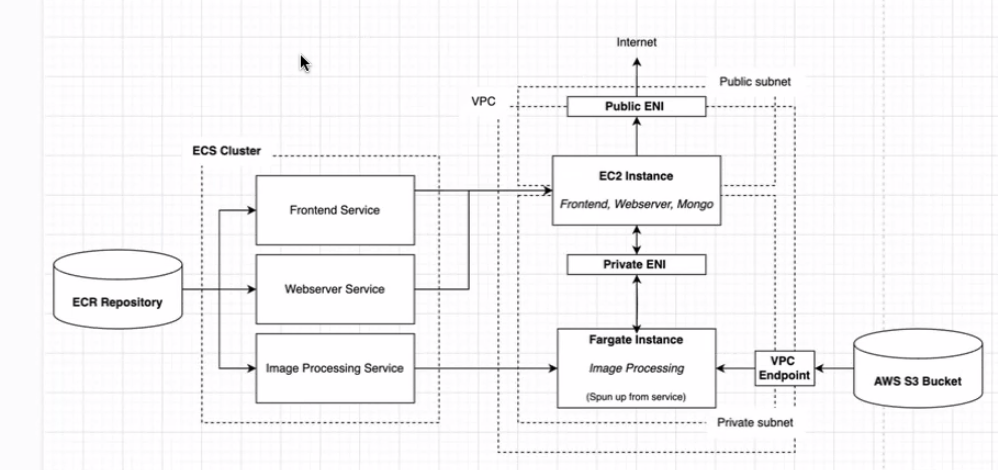
\includegraphics[height=0.7\textheight,width=0.7\textwidth,keepaspectratio]{images/full-mm-infra.png}
\end{frame}

\begin{frame}{Current AWS Infra}
  \centering
  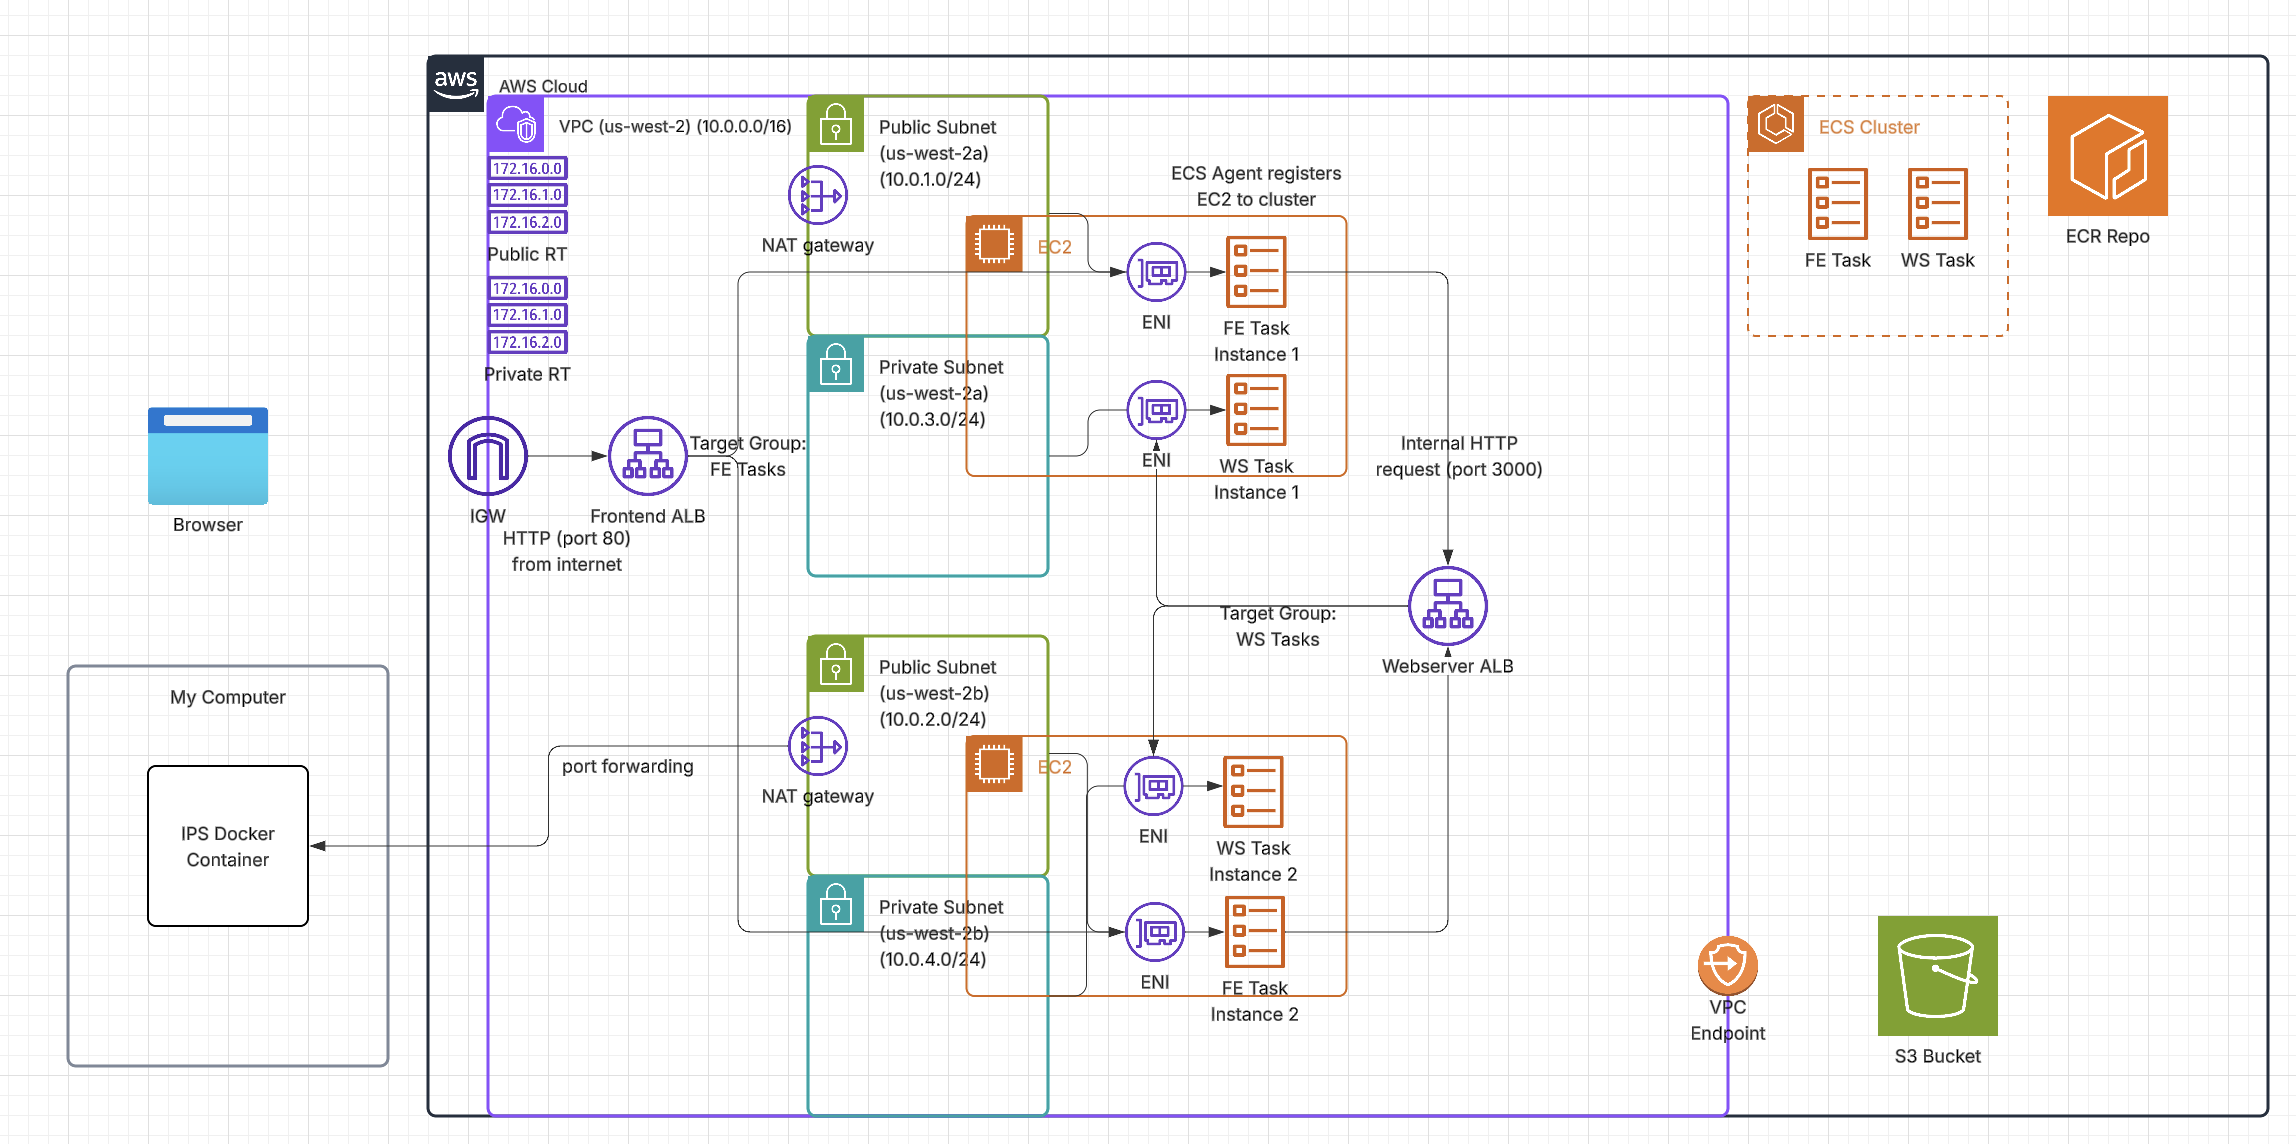
\includegraphics[height=0.7\textheight,width=0.7\textwidth,keepaspectratio]{images/MMICT-ALB-Cloud.png}
\end{frame}

% To create a slide with two columns, use the following:
% \begin{frame}{TITLE}
%     \begin{columns}
%         \begin{column}{0.5\textwidth}
%             COLUMN 1 BODY
%         \end{column}
%         \begin{column}{0.5\textwidth}
%             COLUMN 2 BODY
%         \end{column}
%     \end{columns}
% \end{frame}
